\section{Realisierung}
\label{sec:Realisierung}

TODO: Libraries, Umgebung, Architektur

\subsection{Architektur}

\begin{figure}
    \centering
    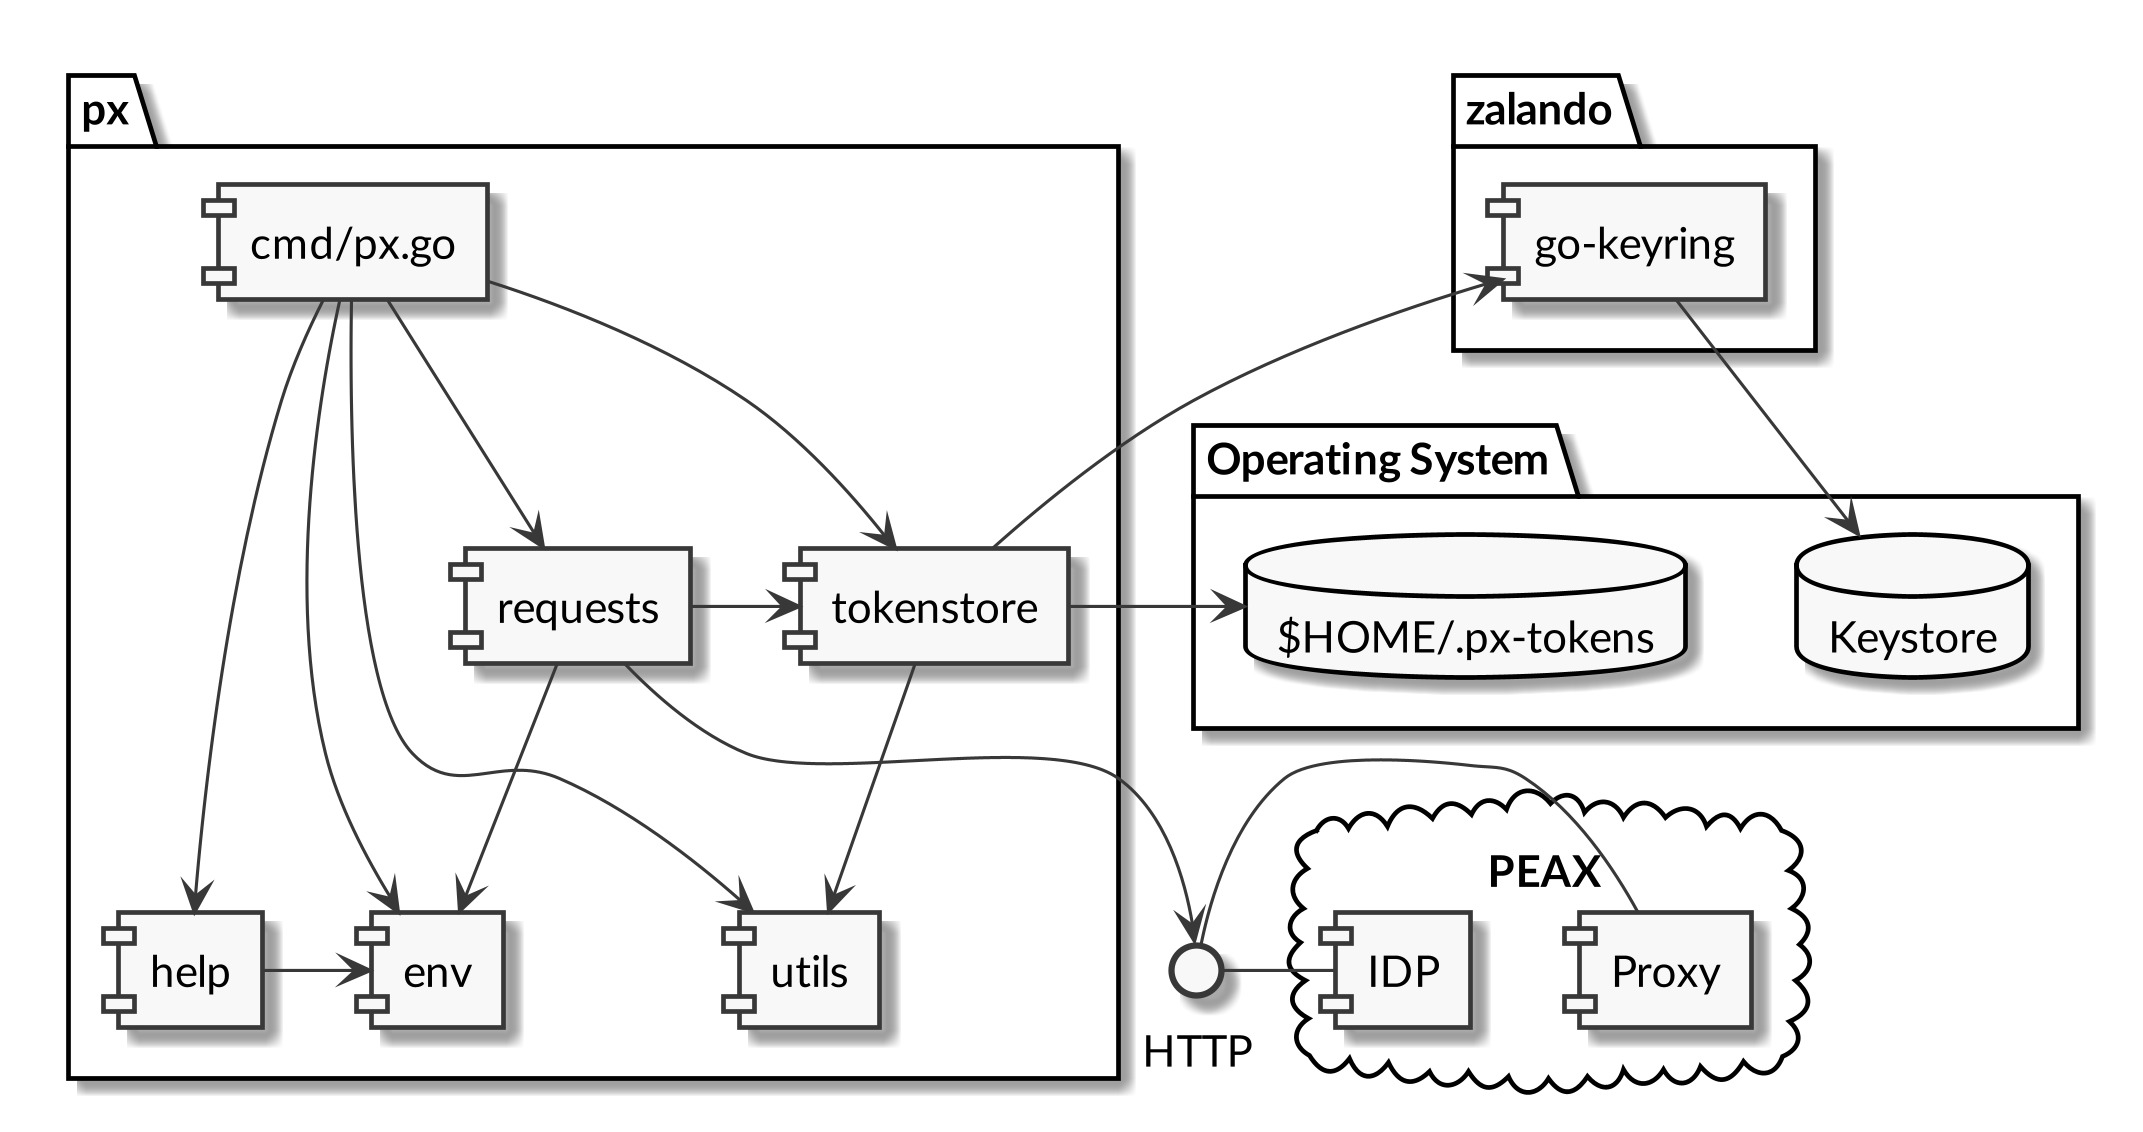
\includegraphics[width=\linewidth]{pics/komponentendiagramm.png}
    \caption{Komponentendiagramm: Die Komponentenarchitektur von \texttt{px}}
\end{figure}

Diese Projektstruktur ist bei \textsc{Go}-Anwendungen weit verbreitet \cite[S. 12]{powerful-cli-apps-in-go}.

\subsection{Befehlsstruktur}

\subsection{Zwei-Faktor-Authentifizierung}

\begin{figure}
    \centering
    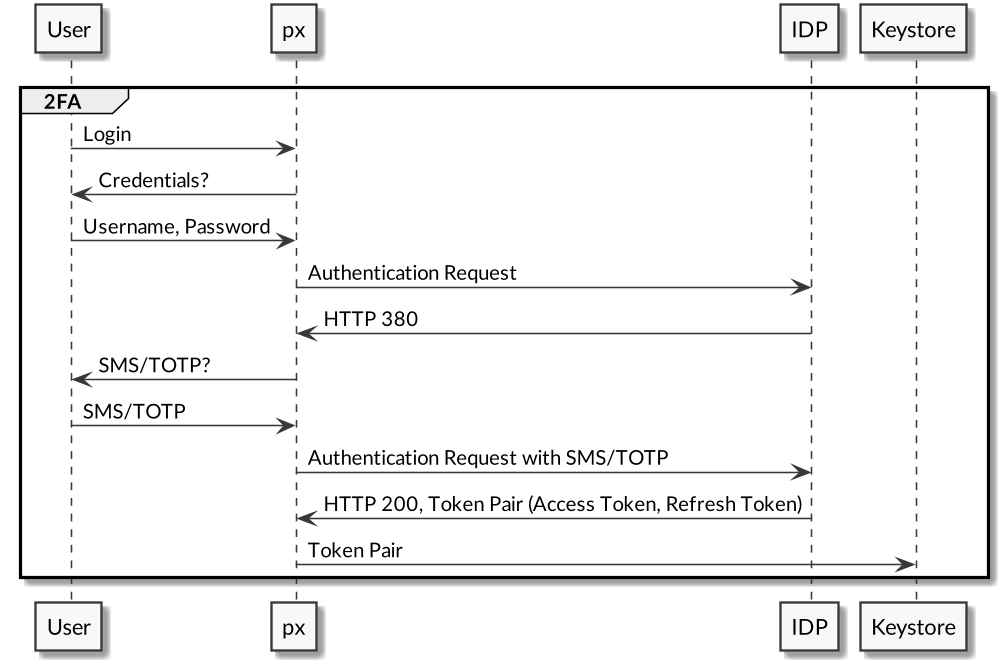
\includegraphics[width=\linewidth]{pics/sequence-2fa.png}
    \caption{Sequenzdiagramm: Der Ablauf der Zwei-Faktor-Authentifizierung mit SMS oder OTP}
\end{figure}

\subsection{Token Store}
\label{sec:realisierung-token-store}

TODO: sicher und unsicher, Datenstruktur

\subsubsection{Fremdkomponente \texttt{zalando/go-keyring}}

\subsection{Retry-Mechanismus}
\label{sec:retry-mechanism}

\begin{figure}
    \centering
    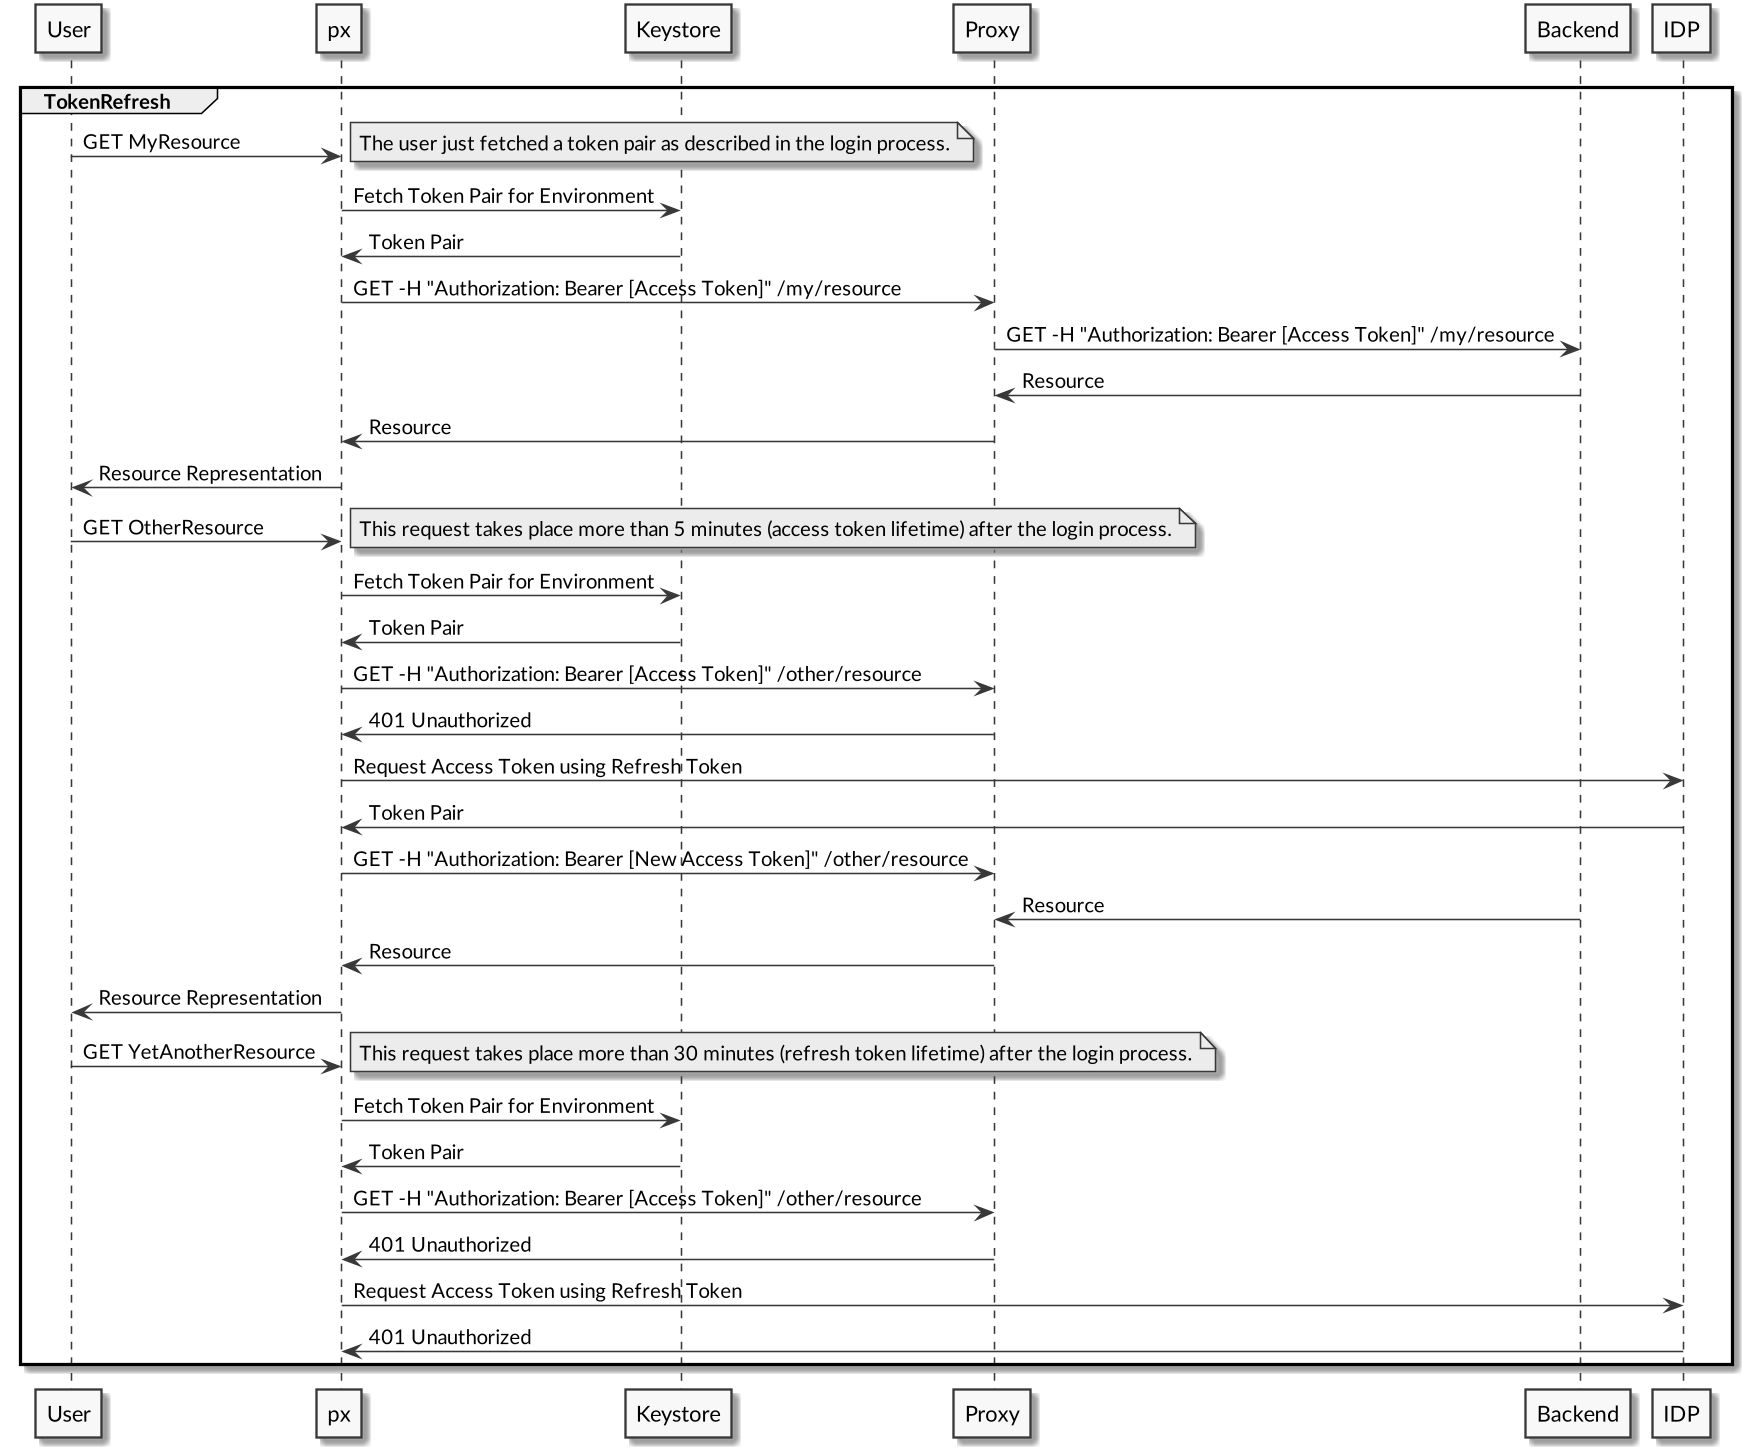
\includegraphics[width=\linewidth]{pics/sequence-retry.png}
    \caption{Sequenzdiagramm: Der für den Benutzer transparente Retry-Mechanismus mit einem Token Pair, das im Hintergrund automatisch aktualisiert wird}
\end{figure}
